 \label{chap:Conceptions}
This chapter contains 2 sections. The first section will cover the process of C++ compilation, including preprocessor, compiler, assembler, link editor and some C++ specialties. The second section will cover JavaScript language, including some of its specialties and its interface with C++. 

\section{C++ compilation process}
    Generally, the process to transform C++ source files into executable file goes through 4 steps \footnotemark. Figure \ref{fig:C++CompilationProcess} shows the general plan of the process of C++ compilation
    
    \begin{enumerate}
        \item The C++ preprocessor reads the source files and  do some prepossessing jobs such as cleaning up the comments, combining lines separate by "\textbackslash"
        into a line, copying the contents of the included header files into the source code file and so on.

        \item The C++ compiler reads the expanded source code files produced previously and then parse and transform them into assembler files for the platform.

        \item The assembler generated object code files/ libraries from the assembler files.

        \item The linker links object code files generated by the assembler together with other preexisting object code files for any library functions used so as to produce an executable file.
    \end{enumerate}
    
    \begin{figure*}
         \centering
        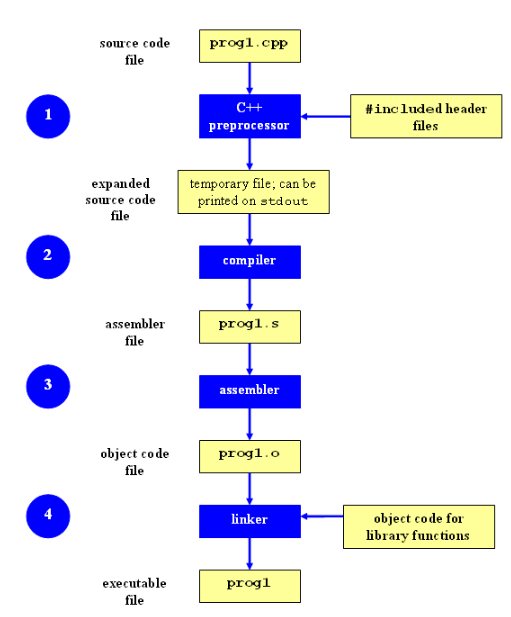
\includegraphics[scale = 0.6]
     {Images/concepts/C++CompilationProcess.png}
        \caption[C++ Compilation Process:]%
    {C++ Compilation Process\footnotemark[\value{footnote}]}
        \label{fig:C++CompilationProcess}
    \end{figure*}
    
    \footnotetext{\url{http://faculty.cs.niu.edu/~mcmahon/CS241/Notes/compile.html}}
    
    \subsection{Preprocessor}
       Before C++ compiler do the parsing job, the preprocessor goes through the following 8 steps:\footnote{\url{https://akaedu.github.io/book/ch21s01.html}} 
           
        \begin{enumerate}
            \item Replace the triplets with the corresponding characters. The corresponding relationship can be found here     \footnote{\url{https://msdn.microsoft.com/en-us/library/bt0y4awe.aspx}}. 
            
               
                    
            \item Combine the lines connected by "\textbackslash" into one line. An example is shown below.
            
                \begin{lstlisting}[language=c, caption= example 1 before]
             #define STR "hello, "\
	            "world"
                \end{lstlisting}
                 
                 \begin{lstlisting}[language=c, caption= example 1 after]
 #define STR "hello, "      "world"
                \end{lstlisting}
                
            
    
            \item Replace the comments (not matter single-line or multi-line notes) by a space.
    
     
            \item After the two steps above removing some of the lines, the remaining lines are called logic code line. Preprocessor then divides the logical lines into Token and space. Tokens are called preprocessing Tokens, including identifiers, integer constants, floating point constants, character constants, strings, operators, and other symbols.\newline 
            For the example given above, the two source lines are concatenated into a logical line of code, which is then divided into Token and space:\newline 
            \textit{\#, define, space, STR, space, "hello," Tab, Tab, "World".}
            
            \item  Identify the preprocessing instructions in the tokens generated previously and do the corresponding jobs. For example, if encounter "\# include" preprocessing instruction, then added the corresponding head files into the source file and repeat step 1 to step 4;  if  encounter a "macro"
            definition, then expand it.
            
            
            \item Find out the constant of char or escape sequence of string, with the corresponding byte to replace it, such as the replacement of "\textbackslash n" by byte 0x0a.
            
            
            \item Concat the adjacent string together. For example, add the following code in example 1.
        
               \begin{lstlisting}[language=c, caption= example 2]
                 printf(
                	STR);
                \end{lstlisting}
                
                After step 4, the tokens will be divided into:\newline 
                \textit{printf, ( , newline, Tab, STR, ), ;, newline}
                
                After step 5, the token STR is expanded into:\newline
                \textit{printf, ( , newline, Tab, "hello", Tab, Tab, "world" ), ;, newline}
              
                And finally, we concat the adjacent string "hello" and "world" in this step:\newline
                \textit{printf, ( , newline, Tab, "hello", "world" ), ;, newline}
                   
            \item Remove all the space and give the rest prepocessing tokens to compiler for grammatical analyse. For the example above, the tokens received by compiler will be: \newline \textit{printf, ( , "hello, world", ), ;}
            
            Tokens in the compiler are renamed as C++ Token.
            
        \end{enumerate}
        
         
        Figure \ref{fig:Preprocessor} gives us a simply illustration of preprocessing.
            
        \begin{figure}
            \centering
            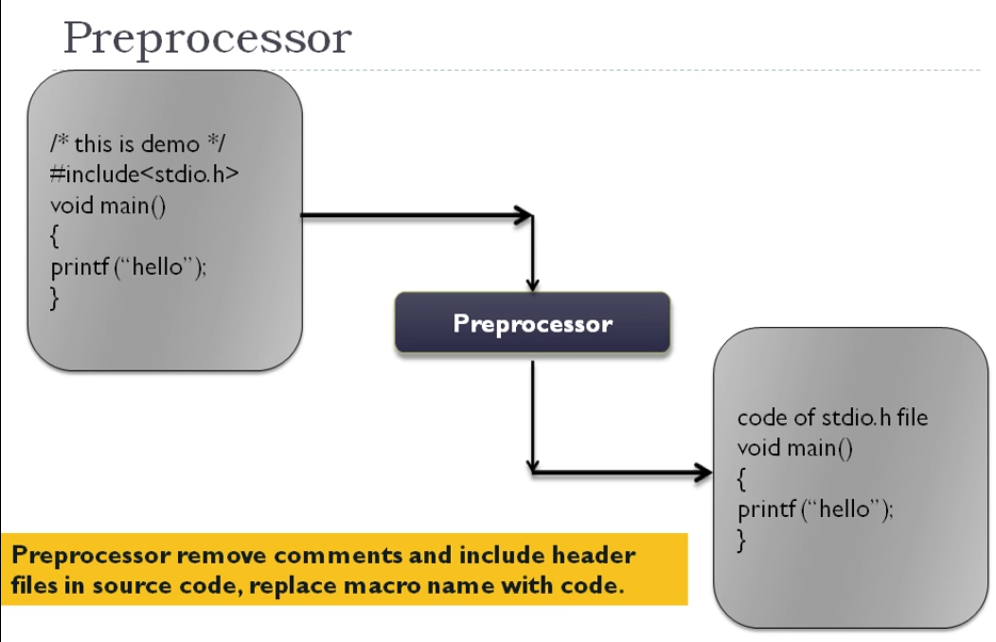
\includegraphics[scale = 0.25]
            {Images/concepts/Preprocessor.png}
            \caption[A simple illustration of preprocessing]%
            {A simple illustration of preprocessing\footnotemark}    \label{fig:Preprocessor}
        \end{figure}
            \footnotetext{\url{https://www.youtube.com/watch?v=VDslRumKvRA}}

            
    
    
    
    \subsection{Compiler}
        Now that we get C++ tokens, the next step is to translate them into assembly. In order to translate one language to another, an abstract syntax tree is needed.  
        
        \subsubsection{Abstract syntax tree}
                    
            As the name implicated, AST is a tree representation of source code syntax at an abstract level. We say this representation is "abstract" because the tree does not show all details, such as semicolons to terminate statements or commas to separate function argument in the real syntax, but the essential characteristics of the structure.\cite {Joel-Jones-03}. Plus, ASTs omit tree nodes representing unary productions in the grammar, because information like that 
    "directly represented in ASTs by the structure of the tree"
    \cite {Joel-Jones-03}.
             
        Here is an example, consider the gramme:
           
           $E \rightarrow int |(E)| E + E $
            
            And the string:
            
            $5+(2+3)$
           
            After preprocessing and lexical analyse, we will get a list of tokens:
            
            $int\textsubscript{5}'+''('int\textsubscript{2}'+'int\textsubscript{3}')'$
            
            
            And we will get a parse tree as shown in figure\ref{fig:parseTree}, that traces the operation of a parser, captures nesting structure, but with too much information such as parentheses and single successor node.  
             \begin{figure}[H]
                \centering
                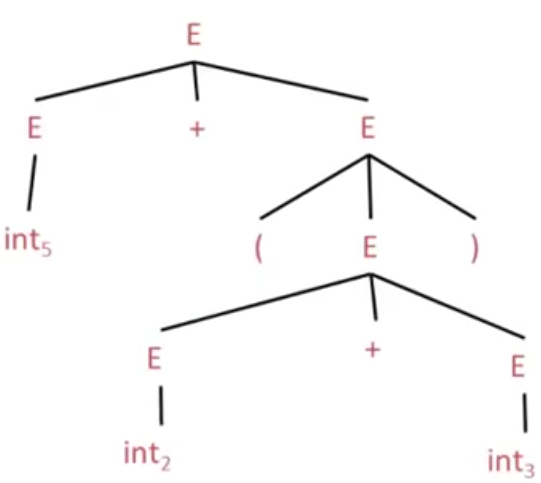
\includegraphics[scale = 0.25]
                {Images/concepts/parseTree.png}
                \caption[ parseTree]%
                { Parse tree\footnotemark}
                \label{fig:parseTree}
            \end{figure}
             \footnotetext{\url{https://www.youtube.com/watch?v=q3idP8tOJIU}}
            
            
            And the abstract syntax tree will like figure \ref{fig:AST}, which also captures the nesting structure but abstract from the concrete syntax. It's more compact and easier to use.
        
             \begin{figure}[H]
                \centering
                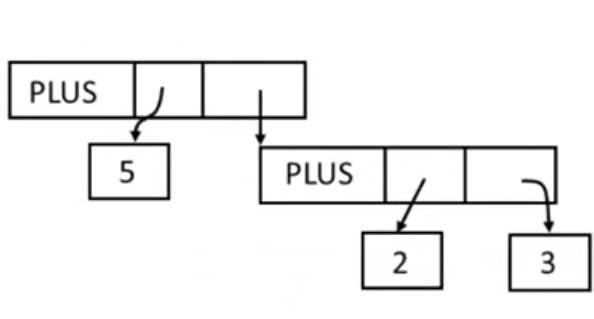
\includegraphics[scale = 0.25]
                {Images/concepts/AST.png}
                \caption[ AST]%
                { Abstract syntax tree\footnotemark}
                \label{fig:AST}
            \end{figure}
             \footnotetext{\url{https://www.youtube.com/watch?v=q3idP8tOJIU}}
             
             
            Now that the abstract syntax tree is obtained, an abstract assembles tree(AAT) and intermediate representation(IR) can be generated. And then from the AAT, an expression tree and a statement tree can be generated. Expression tree defines the "constant", "operator", "register", "memory" and "call" as well as their behaviors of the assembly code. Statement tree defines the "move", "sequential", "call", "label \& jump" as well as their behaviors of the assembly code. Figure \ref{fig:NativeInstruction} gives an overview of the compiling process from an AST to the native machine instruction. 
            
             \begin{figure}
                \centering
                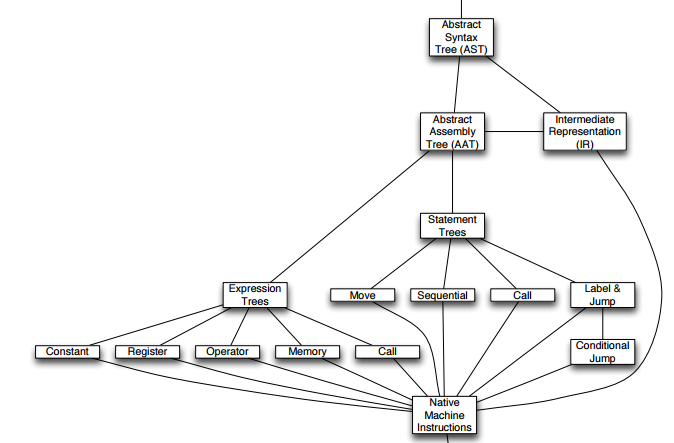
\includegraphics[scale = 0.4]
                {Images/concepts/NativeInstruction.png}
                \caption[From AST to assembly]%
                {From AST to native machine instruction\footnotemark}    \label{fig:NativeInstruction}
            \end{figure}
             \footnotetext{\url{http://www.opensecuritytraining.info/LifeOfBinaries_files/LifeOfBinaries-Map-MediumAndSmall.pdf}}
             
             
             
               \begin{comment}    
                 A simple illustration of Compiling is shown in Figure \ref{fig:Compiler}
        
                    \begin{figure}
                        \centering
                        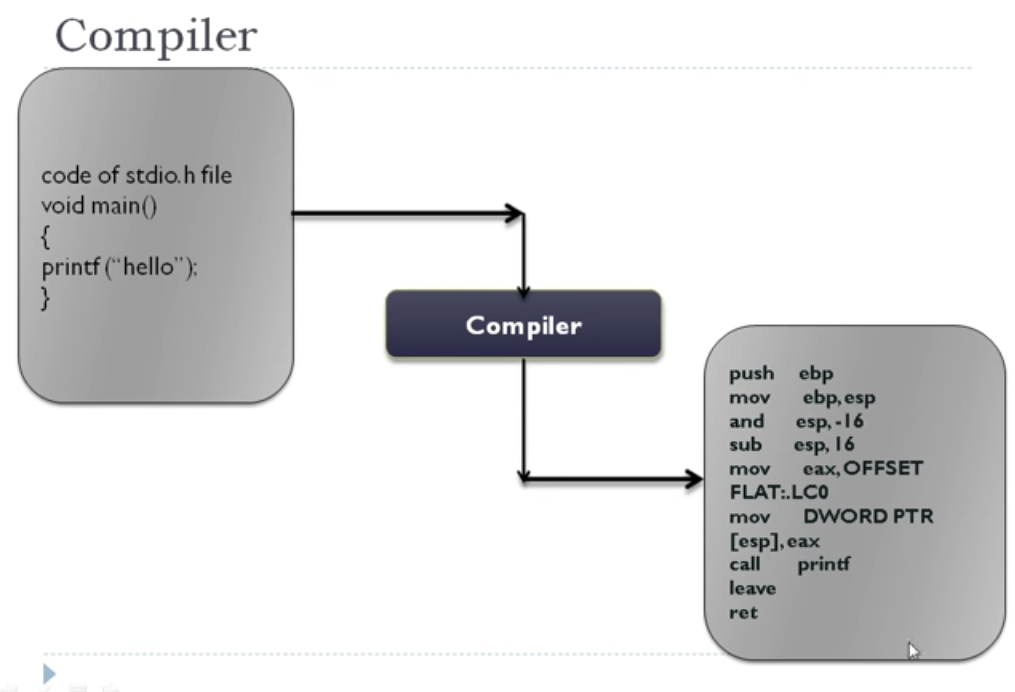
\includegraphics[scale = 0.25]
                        {Images/concepts/Compiler.png}
                        \caption[A simple illustration of compiling]%
                        {A simple illustration of compiling\footnotemark}    
                        \label{fig:Compiler}
                    \end{figure}
                     \footnotetext{\url{https://www.youtube.com/watch?v=VDslRumKvRA}}
             \end{comment}
             
             
             
    \subsection{Assembler} \label{subsection:Assembler}
        In the next step, the assembler code generated by the compiler is assembled into the object code for the platform. Figure \ref{fig:Assembler} gives a simple illustration of this process. The file containing those object code (without modification by link editor) is called relocatable file\cite{TIS-95}, one of the three kinds of the object file. 
        
     
            \begin{figure}[H]
                \centering
                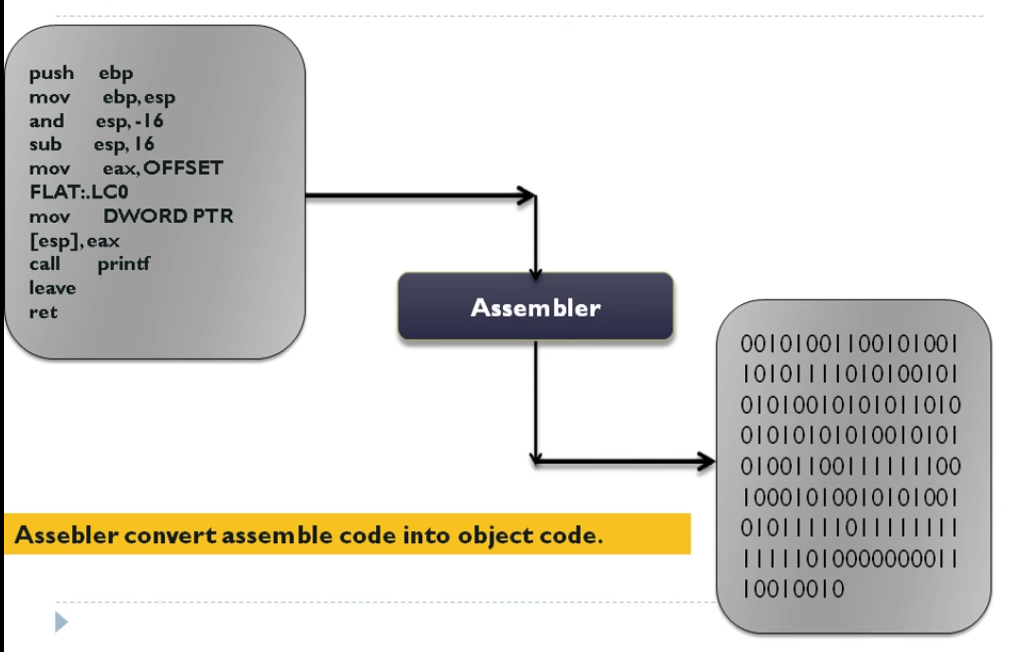
\includegraphics[scale = 0.22]
                {Images/concepts/Assembler.png}
                \caption[A simple illustration of assembling]%
                {A simple illustration of assembling\footnotemark}    
                \label{fig:Assembler}
            \end{figure}
             \footnotetext{\url{https://www.youtube.com/watch?v=VDslRumKvRA}}

        
        \subsubsection{Object files format}
        According to the executable and linkable file (ELF) standard, object files\footnote{I think the author wants to say an executable file here} are binary representations of programs intended to execute directly on a processor\cite{SCO-97}. Programs that require other abstract machines for execution, are excluded, for example shell scripts\cite{SCO-97}. There are three main types of object files.
            
          \begin{enumerate}
                \item Relocatable file: it is used to link with other object files to create an executable or a shared object file. 
                \item Executable file: it holds a program suitable for execution
                \item Shared object file: it is used for linking by link editor firstly, and dynamic linker secondly.
           \end{enumerate}
        
          It deserves mentioning that, Executable files and Shared object files are created altogether by assembler and link editor (see \ref{Link editor}), while Relocatable files can either be generated by an assembler or by an assembler plus link editor\cite{TIS-95}.  
       
        Object files participate in program linking (building a program) and program execution (running a program) \cite{SCO-97}. \textit{For convenience and efficiency, the object file format provides parallel views of a file's contents} \cite{SCO-97}, which is shown in Figure \ref{fig:ELFoverview}. 
        
            \begin{figure}[H]
                \centering
                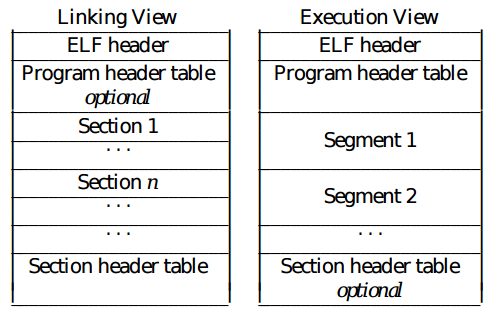
\includegraphics[scale = 0.4]
                {Images/concepts/ELFoverview.png}
                \caption[Object file's organization]%
                {Object file's organization\cite{SCO-97}}    
                \label{fig:ELFoverview}
            \end{figure}
           
        
            At the beginning of an object file is an \textit{ELF header} that holds a "road map" describing the file's organization, for example, a pointer to the program header table and a pointer to the section header table. \textit{Sections} hold the bulk of object file information for the linking view, including instructions, data, symbol table, relocation information, and so on\cite{SCO-97}. \textit{Segments}, on the other hand, contains object file information for the execution view.\textit{program header table} must be presented in the execution files. It tells the system how to create a process image\cite{SCO-97}. \textit{Section header table} must be presented in the relocatable file. It contains information (section name, section size, entry address) describing the file's sections. 
            
            As shown in figure \ref{fig:ELFsections}, a typical complete ELF file contains quite a few sections for code (.text), data (.data), relocation information (.rel.text, .rel.data, and .rel.rodata), linker symbols (.symtab), and debugger symbols (.debe)\cite{LAL-00}. If the file is a C++ program, it will probably also contain .init, .fini, .rel.init, and .rel.fini sections as well\cite{LAL-00}. 
            
            Back to the figure of object file's organization \ref{fig:ELFoverview}, segments are generally made up of one or more related sections. There are some sections, which has nothing to do with execution, that belong to no segment. 
            
            
              \begin{figure}[H]
                \centering
                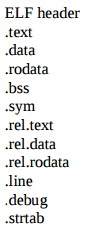
\includegraphics[scale = 0.6]
                {Images/concepts/ELFsections.png}
                \caption[Typicial ELF sections]%
                {Typicial ELF sections\cite{LAL-00}}    
                \label{fig:ELFsections}
            \end{figure}
           
        
            
    \subsection{Link editor}\label{Link editor}        As mentioned in subsection \ref{subsection:Assembler}, an object file is created by assembler and link editor altogether. If an object file is a relocatable file or a shared library file, then it can be linked into an executable file or another library. Figure \ref{fig:Linker} gives a simple overview of this process.         
     \begin{figure}
        \centering
        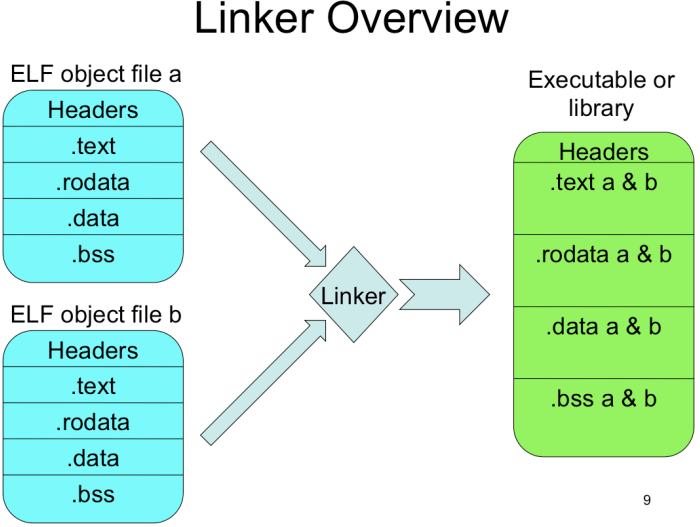
\includegraphics[scale = 0.3]
        {Images/concepts/Linker.png}
        \caption[Linker overview]%
        {Linker overview\footnotemark}    
        \label{fig:Linker}
    \end{figure}
     \footnotetext{\url{http://www.opensecuritytraining.info/LifeOfBinaries_files/2012_LifeOfBinaries3.pdf}}
        
        In order to ensure communication, such as function call between object files generated from different platforms, a standardized interface is needed. And since object files contain binary code, binary level compatibility should be guaranteed. An application binary interface can respond to these needs. It's worth noting that compiler, assembler and link editor, should all follow the guidance of the same ABI to ensure binary compatibility.
        
           \textit{The most obvious and important ABI is that provided by a shared object file since the actual linking is determined at runtime; stability can only be achieved when the library and the applications which use its interfaces adhere to a common stable ABI} \footnote{\url{http://abicheck.sourceforge.net/}}.
        
        \subsubsection{Application binary interface}
            Application binary interface (ABI) describes the interface between two program modules, one of which is often a library or operating system  and the other is an application, at the binary code level. \footnote{\url{https://en.wikipedia.org/wiki/Application\_binary\_interface}}
            Thus, it is ABI that actually determines the binary compatibility between an application and a system.\footnote{\url{http://abicheck.sourceforge.net/}}\newline    
           According to \cite{ALTERA-14}, ABI describes:   
           \begin{enumerate}
              \item  How data is arranged in memory
              \item  Behavior and structure of the stack
              \item  Function calling conventions
            \end{enumerate}
            
        
            
            \paragraph{Data representation}
            When CPU of a machine reads from or writes to memory, it will do that in byte-sized chunks (a byte = 8 bits) rather then bit by bit. If a machine processes data in 4 bytes (32 bits) chunks at a time, we call it a 32 bits machine. Data in memory should be properly aligned so as to improve the performance of a machine. For example, if a machine's word size is 4 bytes, the memory address of data should be located in an address of some multiple of 4. Otherwise, e.g. the data starts at address 14 instead of 16, then the computer has to read two or more 4 byte chunks\footnote{\url{https://en.wikipedia.org/wiki/Data_structure_alignment}}. Even if the previous data structure ends at address 13, the starting point of the next data structure should be at address 16. At addresses 14 and 15, two padding bytes are inserted between the two data structures.
            
            Figure \ref{fig:DataAlign} shows the Intel 386 ABI data alignment policy. Figure \ref{fig:DataAlign1} is an example of using this ABI data alignment. Since the alignment of type "short" is 2 bytes, the starting point of variable "s" is located in address 2 rather than 1. Moreover, one padding byte is added in address 1.
             
              \begin{figure}
                \centering
                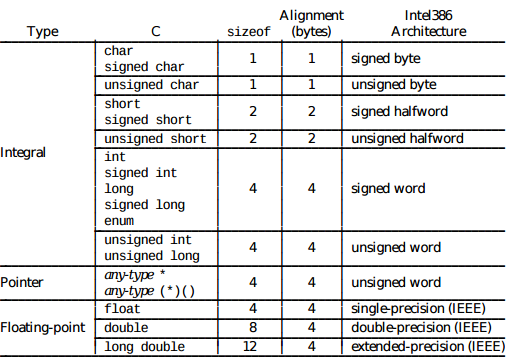
\includegraphics[scale = 0.5]
                {Images/concepts/DataAlign.png}
                \caption[Intel 386 data alignment table]%
                {Intel 386 data alignment table\cite{SCO-386}}    
                \label{fig:DataAlign}
              \end{figure}
              
              
              \begin{figure}
                \centering
                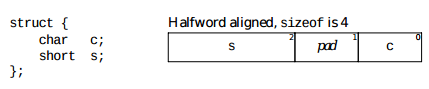
\includegraphics[scale = 0.6]
                {Images/concepts/DataAlign1.png}
                \caption[Intel 386 data alignment example]%
                {Intel 386 data alignment example\cite{SCO-386}}    
                \label{fig:DataAlign1}
              \end{figure}
            
            
        \paragraph{Function calling convention}
        The ABI's function calling convention describes stack frame layout, register usage, parameter passing, and so on. Libraries require this calling sequence\cite{SCO-386}.
        
        Generally, every processor in a computer has some registers that part of them are global to all procedures in a running program. Figure shows\ref{fig:Register} the global registers of intel 386.
        
            \begin{figure}[H]
                \centering
                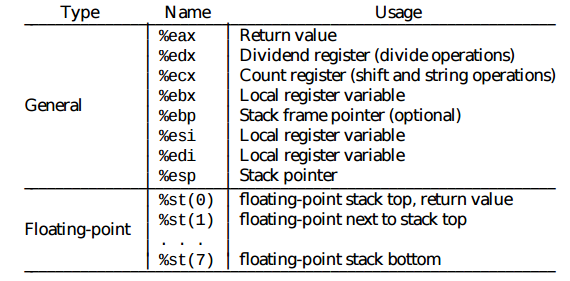
\includegraphics[scale = 0.4]
                {Images/concepts/Register.png}
                \caption[Intel 386 global register]%
                {Intel 386 global register\cite{SCO-386}}   
                \label{fig:Register}
            \end{figure}
            
            
        In addition to registers, each function has a frame on the run-time stack that grows downward from high addresses\cite{SCO-386}, as shown in figure \ref{fig:FunctionStack}.
        
        
            \begin{figure}
                \centering
                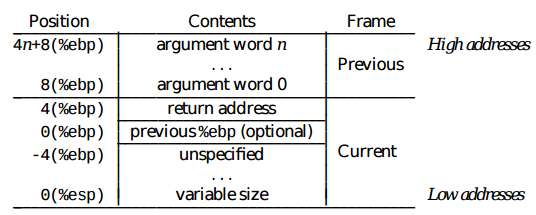
\includegraphics[scale = 0.4]
                {Images/concepts/FunctionStack.png}
                \caption[Intel 386 function run-time frame]%
                {Intel 386  function run-time frame\cite{SCO-386}}   
                \label{fig:FunctionStack}
            \end{figure}
            
        There are 4 key points about the stack frame that worth noting.
        
            \begin{enumerate}
                \item The stack is aligned in word.
                \item Argument words are pushed onto the stack from right to left (that is, the rightmost argument in C call syntax has the highest address), and remains the stack's word alignment\cite{SCO-386}. Every input arguments appear on the stack will reside
                in the stack frame of the caller \cite{SCO-386}.
                \item An argument's size can be increased, to ensure it has a size of multiple of words.
                \item There is no limit of a maximum stack frame size.
            \end{enumerate}
            
        All the global registers are visible to both a calling and a called function. Thus, a called function must preserve these register's values for its calling function, which is illustrated in figure \ref{fig:FCCPrologue}.   
        
               \begin{figure}[H]
                    \centering
                    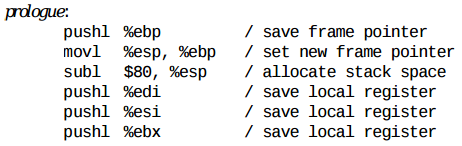
\includegraphics[scale = 0.5]
                    {Images/concepts/FCCPrologue.png}
                    \caption[Function calling convention prologue]%
                    {Function calling convention prologue\cite{SCO-386}}    
                    \label{fig:FCCPrologue}
              \end{figure}
        
        After this preparation, a processor can start calling a function. In the assembly code, the \textit{call} instruction will firstly push the address of the next instruction (the return address) onto the calling function's stack frame. And then, it passes the control right to the called function. As described earlier, the called function must firstly preserve the caller's registers. After that, the main logic is executed. And some cleaning up jobs such as restoring the initial values of the caller's registers, putting the return value into \%eax register, etc. Finally, the called function will be terminated by a \textit{ret} instruction that pops the address (the returning address for its caller) off the stack as shown in figure \ref{fig:FCCepilogue}. 
        
               \begin{figure}[H]
                    \centering                    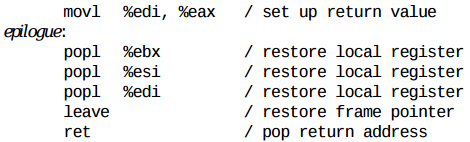
\includegraphics[scale = 0.5]
                    {Images/concepts/FCCepilogue.png}
                    \caption[Function calling convention epilogue]%
                    {Function calling convention epilogue\cite{SCO-386}}    
                    \label{fig:FCCepilogue}
              \end{figure}
              
       The control right is now back to the calling function and the processor continues execution at the next instruction after the call instruction. Figure \ref{fig:FCCret} illustrates the stack contents after \textit{call} instruction and \textit{ret} instruction.
       
               \begin{figure}[H]
                    \centering
                    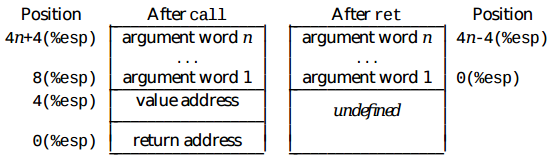
\includegraphics[scale = 0.45]
                    {Images/concepts/FCCret.png}
                    \caption[Stack contents for function call]%
                    {Stack contents for function call\cite{SCO-386}}    
                    \label{fig:FCCret}
              \end{figure}
              
       \subsubsection{Static link}
       One of the most essential jobs of every modern linker is to handle libraries\cite{LAL-00}. In this part we cover traditional statically linked libraries, leaving the more complex shared libraries next. 
       
       \paragraph{Two-pass linking}
       In order to create a static link library, a linker will go through a process called two-pass linking.
       
       In the first pass, a linker takes as its input a set of input object files, libraries, and perhaps command files, and produces as its result an output object file\cite{LAL-00}.When a linker runs, it first has to find the sizes of the segments by scanning the input files. And then it collects the definitions and references of all of the symbols. It creates a segment table that lists all of the segments defined in the input files, and a symbol table with all of the symbols imported or exported\cite{LAL-00}.
       
        In the second pass, a linker uses information collected in the first pass to control the actual linking process\cite{LAL-00}. It reads and relocates the object code, and replace symbol references with numeric addresses. Then it adjusts memory addresses in code and data (by referring to segments such as .rel.data, .rel.text ) to reflect relocated segment addresses, and writes the relocated code to the output file\cite{LAL-00}. Finally, the linker writes the output file, which generally holding header information, relocated segments, and symbol table information\cite{LAL-00}.
      
       
       The following example illustrates in detail the process of static link, including the usage of some Linux commands for compiling and linking code and reading ELF files.\newline
       
       \textbf{A.} Create two source file called "common.c" and "test.c" as below.
       
       
            \begin{lstlisting}[language=c, caption= common.c]
    int val = 1; 
    
    int func(void) 
    { 
        return (val+10); 
    } 
            \end{lstlisting}
                
       
            \begin{lstlisting}[language=c, caption= test.c]  
    extern int val; 
    extern int func(void); 
    
    int main() 
    { 
        val = 10; 
        func(); 
        return 0; 
    }                
            \end{lstlisting}  
            
        \textbf{B.} Compile them into object files by using command: \textit{gcc -c test.c} and \textit{gcc -c common.c}. After this step, we will get "test.o" and "common.o" files. All of them are relocatable files as they haven't been modified by any linker (we can verify this by using the command \textit{readelf -h --filename} to read the files' headers).\newline
        
        
        
        \textbf{B1.text.o}
        Use command \textit{readelf -s test.o} to read the symbol table of "test.o" and we will get the following result. 
        
        \begin{lstlisting}[caption= Symbol table of "test.o"]
Symbol table '.symtab' contains 11 entries: 
   Num:    Value          Size Type    Bind   Vis      Ndx Name 
     0: 0000000000000000     0 NOTYPE  LOCAL  DEFAULT  UND 
     1: 0000000000000000     0 FILE    LOCAL  DEFAULT  ABS test.c 
     2: 0000000000000000     0 SECTION LOCAL  DEFAULT    1 
     3: 0000000000000000     0 SECTION LOCAL  DEFAULT    3 
     4: 0000000000000000     0 SECTION LOCAL  DEFAULT    4 
     5: 0000000000000000     0 SECTION LOCAL  DEFAULT    6 
     6: 0000000000000000     0 SECTION LOCAL  DEFAULT    7 
     7: 0000000000000000     0 SECTION LOCAL  DEFAULT    5 
     8: 0000000000000000    26 FUNC    GLOBAL DEFAULT    1 main 
     9: 0000000000000000     0 NOTYPE  GLOBAL DEFAULT  UND val 
    10: 0000000000000000     0 NOTYPE  GLOBAL DEFAULT  UND func
         \end{lstlisting}      
        
        Since \textit{val} and \textit{func} are not defined in test.c, the Ndx (index of the section where the symbol is located) of these two symbols is UND. In order to make sure this program to run successfully, we hope that these two symbols can be found in other files and their addresses can be determined in the linking process. To determine the address of an undefined symbol is called relocation.\newline
        
        Use command \textit{readelf -S test.o}to read the section header table of "test.o". 
        
        \begin{lstlisting}[caption=Section header table of "test.o"]
here are 12 section headers, starting at offset 0x128: 

Section Headers: 
  [Nr] Name              Type             Address           Offset 
       Size              EntSize          Flags  Link  Info  Align 
  [ 0]                   NULL             0000000000000000  00000000 
 0000000000000000           0     0     0 
  [ 1] .text             PROGBITS         0000000000000000  00000040 
       000000000000001a  0000000000000000  AX       0     0     4 
  [ 2] .rela.text        RELA             0000000000000000  00000548 
 0000000000000018          10     1     8 
  [ 3] .data             PROGBITS         0000000000000000  0000005c 
 0000000000000000  WA       0     0     4 
  [ 4] .bss              NOBITS           0000000000000000  0000005c 
 0000000000000000  WA       0     0     4 
  [ 5] .comment          PROGBITS         0000000000000000  0000005c 
       000000000000002d  0000000000000001  MS       0     0     1 
  [ 6] .note.GNU-stack   PROGBITS         0000000000000000  00000089 
 0000000000000000           0     0     1 
  [ 7] .eh_frame         PROGBITS         0000000000000000  00000090 
 0000000000000000   A       0     0     8 
  [ 8] .rela.eh_frame    RELA             0000000000000000  00000578 
 0000000000000018          10     7     8 
  [ 9] .shstrtab         STRTAB           0000000000000000  000000c8 
 0000000000000000           0     0     1 
  [10] .symtab           SYMTAB           0000000000000000  00000428 
 0000000000000018          11     8     8 
  [11] .strtab           STRTAB           0000000000000000  00000530 
 0000000000000000           0     0     1 
Key to Flags: 
  W (write), A (alloc), X (execute), M (merge), S (strings) 
  I (info), L (link order), G (group), x (unknown) 
  O (extra OS processing required) o (OS specific), p (processor specific)
        \end{lstlisting}
        
       From the description of rela.text, we find link = 10, info = 1. link = 10 represents the index of the symbol that will be relocated in the symbol table; info = 1 represents the index of the section that will be relocated (in our example is ".text" section).\newline
       
       More relocation information can be found using command \textit{readelf -r test.o}
        
        \begin{lstlisting}[caption=Relocation section of "test.o"]
Relocation section '.rela.text' at offset 0x548 contains 2 entries: 

Offset          Info           Type           Sym. Value    Sym. Name + Addend 

000000000006  000900000002 R_X86_64_PC32     0000000000000000 val - 8 

00000000000f  000a00000002 R_X86_64_PC32     0000000000000000 func - 4 

Relocation section '.rela.eh_frame' at offset 0x578 contains 1 entries: 

Offset          Info           Type           Sym. Value    Sym. Name + Addend 

 000200000002 R_X86_64_PC32     0000000000000000 .text + 0            \end{lstlisting}
            
         
    "Offset" indicates the offset of the symbol in the relocated section, the higher 4 bytes of "info" indicates the index of the symbol in ".symtab", the lower 4 bytes indicates the type of relocation, and the method of calculating the destination address depends on the "Type".
    In summary, we can obtain information of symbol "val" and "func" as following:
    \begin{enumerate}
        \item Relocation address of "val" is in the section ".text" with an offset of 6. In the future linking process, the linker will write the address of "val" into this relocation address.
        \item Symbol "val" can be found in section ".symtab" with an offset of 9.
        \item  Relocation address of "Func" is in the section ".text" with an offset of 0xf. In the future linking process, the linker will write the address of "Func" into this relocation address.
        \item Symbol "Func" can be found in section ".symtab" with offset of 0xa.
    \end{enumerate}
   
     Since the relocation type of "val" and "func" are both "R\_X86\_64\_PC32",the method to calculate their relocation address is "S+A-P", which is the "symbol address" subtracts the "address of the next instruction"\cite{TIS-95}.\newline
     
     Use command \textit{objdump -S test.o} to disassemble the "test.o file". We will get the following result.
     \begin{lstlisting}[caption=Disassembly of section .text: ]
<main>: 
   0:    55                       push   %rbp 
   1:    48 89 e5                 mov    %rsp,%rbp 
   4:    c7 05 00 00 00 00 0a     movl   $0xa,0x0(%rip)        # e <main+0xe> 
   b:    00 00 00 
   e:    e8 00 00 00 00           callq  13 <main+0x13> 
  13:    b8 00 00 00 00           mov    $0x0,%eax 
  18:    c9                       leaveq 
  19:    c3                       retq
     \end{lstlisting}
     
     As shown in the result, the four bytes (the address of the val) at offset 6 in the ".text" section are all zeros and the four bytes at offset f (the address of func) are also all zeros.
     
     
    \textbf{B2.common.o}
    Here we go through the same way as the analyse of "test.o" and some details will be omitted.
    Use \textit{readelf -s common.o} to read the symbol table.
    \begin{lstlisting}[caption = Symbol table of common.o]
    ...
8: 0000000000000000     4 OBJECT  GLOBAL DEFAULT    3 val 
9: 0000000000000000    15 FUNC    GLOBAL DEFAULT    1 func    
    \end{lstlisting}
    "val" is in index 3 and "func" is in index 1; both of them are defined inside "common.o"\newline
        
    Read its section header table with command: \textit{readelf -S common.o}
    \begin{lstlisting}[caption = Section header table of common.o]
    ......
[ 2] .rela.text        RELA             0000000000000000  00000528 
       0000000000000018  0000000000000018          10     1     8 
......
    \end{lstlisting}
    We can see the section ".text" needs to be relocated.\newline
    
    
    More detail for relocation information with command:\textit{readelf -r common.o}
     \begin{lstlisting}[caption = Relocation section  of common.o]
Relocation section '.rela.text' at offset 0x528 contains 1 entries: 
  Offset          Info           Type           Sym. Value    Sym. Name + Addend 
  
000000000006  000800000002 R_X86_64_PC32     0000000000000000 val - 4 
...
     \end{lstlisting}
    From the information above, symbol "val" should be relocated with the type "R\_X86\_64\_PC32". The relocated address will be placed into the address of section ".text" with offset 6. \newline
    
    
    Disassemble common.o with command: \textit{Objdump -S common.o}
    \begin{lstlisting}[caption = Disassemble common.o]
    ......
0000000000000000 <func>: 
   0:    55                       push   %rbp 
   1:    48 89 e5                 mov    %rsp,%rbp 
   4:    8b 05 00 00 00 00        mov    0x0(%rip),%eax        # a <func+0xa> 
   a:    83 c0 0a                 add    $0xa,%eax 
   d:    c9                       leaveq 
   e:    c3                       retq 
   ......
    \end{lstlisting}
    
    The address with offset 6 (address of "val") are all zeros, which will be replaced by a proper address after relocation.\newline
    
    \textbf{C.} Link "test.o" and "common.o" together with command: \textit{gcc -o test test.o common.o}. The file "test.o" becomes an "EXEC" file. Now, all of the symbols that needed to be relocated (in our example "val" and "func") are properly filled with their final address. 
    
    Disassemble "test" with command: \textit{objdump -S test > test.S}
    \begin{lstlisting}[caption = Disassemble "test" ]
    ......
<main>: 
  400474:       55                      push   %rbp 
  400475:       48 89 e5                mov    %rsp,%rbp 
  400478:       c7 05 ca 03 20 00 0a    movl   $0xa,0x2003ca(%rip)        # 60084c <val> 
  40047f:       00 00 00 
  400482:       e8 09 00 00 00          callq  400490 <func> 
  400487:       b8 00 00 00 00          mov    $0x0,%eax 
  40048c:       c9                      leaveq 
  40048d:       c3                      retq 
  40048e:       90                      nop 
  40048f:       90                      nop 

0000000000400490 <func>: 
  400490:       55                      push   %rbp 
  400491:       48 89 e5                mov    %rsp,%rbp 
  400494:       8b 05 b2 03 20 00       mov    0x2003b2(%rip),%eax        # 60084c <val> 
  40049a:       83 c0 0a                add    $0xa,%eax 
  40049d:       c9                      leaveq 
  40049e:       c3                      retq 
  40049f:       90                      nop 
......
    \end{lstlisting}
    
     From the result above, relocation takes place in the address "400478", "400482" and "400494". They represent the address of "val" and "func" in "test" and "val" in "common.o" respectively. 
     
     Take "val" in "test" file (the line begin with the address "400478") as an example to check whether the relocated address is the same as predict. 
     
     \begin{lstlisting}[caption = Relocation address calculation ]
400478:       c7 05 ca 03 20 00 0a    movl   $0xa,0x2003ca(%rip)        # 60084c <val> 
40047f:       00 00 00 
400482:       e8 09 00 00 00          callq  400490 <func> 
     \end{lstlisting}
     
     It's mentioned previously that for type "R\_X86\_64\_PC32", the relocation address can be calculated by using "symbol address" to subtract "address of next instruction". We can find from the assemble code above that symbol address for "val" in the "text" file is "0x60084c"; the next instruction "callq" begins with the address "0x400482". So the relocated address should be:    
     
     \textbf{0x60084c - 0x400482 = 0x2003ca}
     
     That's exactly the same number in address of section ".text" with offset 6 (read the line "400478" from right to left).
     
     
     Now, the whole process of static linking is finished. In the next part, the dynamic linking will be discussed.  
     
        
    \subsubsection{Dynamic link}
    The problem with static link is the code duplication. If "program1" and "program2" both use a library called "common.o", the commonly used library will be compiled into these two programs respectively. If we have 100 common libraries used by 100 programs, that will be a huge waste of storage space. The mechanism of dynamic linking delays much of the linking process until a program start running\cite{LAL-00}, which means these common (shared) libraries will not be compiled into the final executable file. 
    
    When building an executable file that uses dynamic linking, the link editor adds a program header element of type PT\_INTERP to the executable file\cite{TIS-95}. So that the system knows it needs to invoke the dynamic linker\cite{TIS-95}. The link editor also constructs a number of data that helps the dynamic linker to link executable and shared object files\cite{TIS-95} such as the ".dynamic", ".got" and ".plt" sections. It's shown in figure \ref{fig:ELFsharedlibrary}.
    
            \begin{figure}
                \centering
                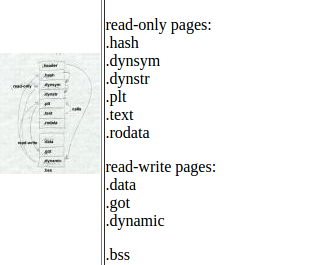
\includegraphics[scale = 0.6]
                {Images/concepts/ELFsharedlibrary.png}
                \caption[An entire ELF shared library]%
                {An entire ELF shared library\footnotemark}    
                \label{fig:ELFsharedlibrary}
            \end{figure}
            
            \footnotetext{\url{http://www.iecc.com/linker/linker10.html}}
        
    En brief, the process of dynamic linking can be described in 3 steps:
        \begin{enumerate}
            \item Bootstrap dynamic linker
            \item Load all necessary shared libraries
            \item Relocation and initialisation
        \end{enumerate}
      
        \paragraph{Dynamic linker}        
        Dynamic linker itself is also a shared library, but it's special. Generally, the relocation of shared libraries is done by the dynamic linker and they can use other shared libraries as well\cite{LAL-00}. However, the dynamic linker can not rely on any other shared library and it needs to self-relocate. How the dynamic linker bootstrap is beyond our discussion.
        
        \paragraph{Load shared libraries}
        After the dynamic linker bootstrap, it collects symbols from the executable file and combines them into a global symbol table so as to find out which shared libraries are required\cite{LAL-00}. As mentioned previously, with the help of ".dynamic" section (added by link editor), the dynamic linker can find out all necessary shared libraries. It then loads these shared libraries according to their dependency. Every newly loaded shared library's symbols are added into the dynamic linker's global symbol table\cite{LAL-00}.
    
        \paragraph{Relocation and initialisation}
        Since the dynamic linker has the global symbol table, it starts traversing relocation tables of the executable file as well as all depending shared libraries and relocate their "GOT/PLT" part to the proper address (the details of relocation is not discussed because of the limite of time)\cite{LAL-00}. After relocation, if a shared library has a section ".init", the dynamic linker will execute those code for initialisation. If a shared library has a ".fini" section, the dynamic linker will execute those code when a process exits\cite{LAL-00}.  
        
        
        \paragraph{Lazy procedure linkage (PLT)}
        Generally, a shared library contains a lot of functions but only a few of them are used in a single run of the program\cite{LAL-00}. Besides, shared functions used in error routines or other parts of the program may never be called\cite{LAL-00}. Furthermore, most of the shared library contain calls to functions that are defined in other static or dynamic libraries. As these functions are neither called directly nor indirectly by the program, fewer of them will be executed in a single program run\cite{LAL-00}.
                
        In order to speed up a program's start, dynamically linked ELF programs use lazy binding of procedure addresses\cite{LAL-00}. Namely, only when an executable file runs to the part where there are symbols defined by shared libraries, will the dynamic linker relocate these symbols.
        
        
        
        %http://www.iecc.com/linker/linker10.html
        %http://www.opensecuritytraining.info/LifeOfBinaries_files/2012_LifeOfBinaries3.pdf
    
    \subsection{C++ features}
        Binary level compatibility of C++ program is difficult to achieve because of the various features of C++u are very complex. In this part, we will explain why it's difficult to support features such as "Template", "Virtual function" as well as "overloading". 
        
        \subsubsection{Template and virtual functions}
        C++ supports "Template" and "Virtual function" features. An environment in which all of the parts of a program are processed simultaneously is implicitly required for those features\cite{LAL-00}. And this will result in a huge number of duplicated code. For example , if different source files of a program that all of them use template "T" and are compiled in a different time, then each of the generated object files will have a copy of template "T"'s binary code. Because when a source file is being compiled, the linker doesn't know whether another source file of the same program has compiled the template or not, so the most straight straightforward solution is to make the duplication. It's the same for virtual functions. For a C++ class that uses virtual functions, it must have virtual function table (vtbl) containing the addresses of all the virtual functions \cite{LAL-00}. So, when source files using the same virtual function are compiled in a different time, there will be a duplication of the "vtbl". 
        
        \textit{Many recent C++ systems have addressed the problem head-on, either by making the linker smarter, or by integrating the linker with other parts of the program development system.}\cite{LAL-00}. Since C++ doesn't have a binary level standard, different systems and different compilers will behave in quite a different way. That's also why the binary level compatibility is difficult to achieve for C++ as mentioned previously.
        
        
        
        \subsubsection{Overloading}
        One of the special features of C++ is overloading, which means a programmer can define many functions and variable with the same name but with different scopes for variables and with different argument types (number as well) for functions. 
        
        In order to support this feature, those overloading functions and variable in source file should be mapped into unique names according to their scopes or arguments when they are compiled into files. By doing so, the link editor can then identify all these symbol properly. This process is called name mangling\cite{LAL-00}.
        
        Figure \ref{fig:nameMangling} lists the rules of how to represent different argument types for an overloading function.
        For example, if we have a function like this in source code:
        
        \begin{lstlisting}[caption = function in source file before name mangling]
    func(int, double) 
        \end{lstlisting}
        
        After mangling, it will become:
        
        \begin{lstlisting}[caption = function in object file after name mangling]
    func__Fid 
        \end{lstlisting}
        
        
        \begin{figure}[H]
            \centering
            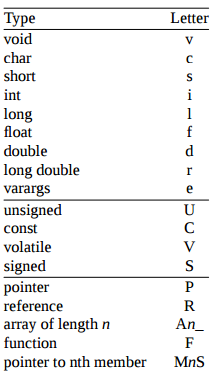
\includegraphics[scale = 0.6]
            {Images/concepts/namemangling.png}
            \caption[Intel 386 function run-time frame]%
            {Intel 386  function run-time frame\cite{LAL-00}}  
            \label{fig:nameMangling}
        \end{figure}
        
    Figure \ref{fig:nameMangling} shows only a little part of all the rules for mangling and the example above is only a very simply illustration. In reality, there are far more rules to define the process of name mangling. 
        
    
\section{JavaScript}

    JavaScript is a lightweight, interpreted, script language with first-class functions supporting prototype based object construction. \footnote{\label{foot:MDN1}\url{https://developer.mozilla.org/en-US/docs/Web/JavaScript}}. It can be used for procedural and object oriented programming \textsuperscript{\ref{foot:MDN1}}. Same as other scripting languages, JavaScript doesn't need compiling before being run\footnote{\label{foot:w3}\url{https://www.w3.org/standards/webdesign/script}}. The major application of JavaScript is in the context of a Web browser and the other common application is as a server side scripting language, for example, in Node.js \textsuperscript{\ref{foot:MDN1}}. In order to reduce the new concepts for learning a language, JavaScript uses basic syntax which is intentionally similar to both Java and C++ \footnote{\label{foot:MDN2}\url{https://developer.mozilla.org/en-US/docs/Web/JavaScript/About\_JavaScript\#JavaScript\_resources}}.
    
    \subsection{JavaScript engine}
    A JavaScript engine is a virtual machine that supposed to execute JavaScript code. For the historical reason of browser wars, now we have many different JavaScript engines such as "SpiderMonkey" that powers FireFox, "V8" that developed by Google and used by Chrome as well as NodeJs, "JavaScriptCore" that developed by Apple for Safari and "Chakra" for IE of Microsoft\footnote{\url{https://en.wikipedia.org/wiki/JavaScript_engine}}. These engines execute JavaScript in a quite different way.Since this project uses NodeJs as its JavaScript executing environment, only V8 engine is discussed.
    
    \paragraph{V8 engine} V8 is a high-performance JavaScript engine written in C++ and open source\footnote{\label{foot:v8git}\url{https://github.com/v8/v8/wiki}}. It consists of two compilers that compile source code directly into machine code: one is "Full-codegen" and the other is "Crankshaft"\footnote{\label{foot:v8Intro}\url{http://developer.telerik.com/featured/a-guide-to-javascript-engines-for-idiots/}}."Full-codegen" is fast but only generates unoptimized code. On the contrary, "Crankshaft" is slow and produces fast, optimized code. Figure \ref{fig:V8compiler} is an illustration of this process.
    
        \begin{figure}[H]
            \centering
            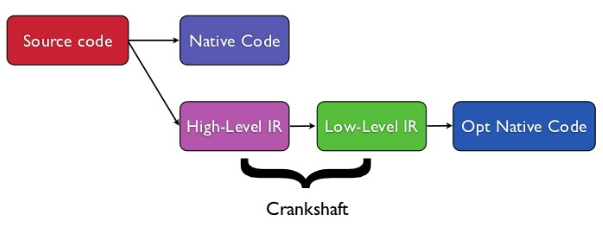
\includegraphics[scale = 0.4]
            {Images/concepts/v8.png}
            \caption[V8compiler]%
            {V8 compiler\footnote{\url{http://www.slideshare.net/nwind/virtual-machine-and-javascript-engine/66-Builtin_objects_written_in_JSfunction}}}  
            \label{fig:V8compiler}
        \end{figure}
        
    In fact, these two compilers are generally used together. "Full-codegen" produces the unoptimized native code, and then "crankshaft" determines whether the generalized code needs to be optimized\textsuperscript{\ref{foot:v8Intro}}. If yes, "Crankshaft" produces code after optimization and replaces the old one\textsuperscript{\ref{foot:v8Intro}}. Figure \ref{fig:crankshaft} is the overview work-flow of crankshaft. In this optimizing process, "crankshaft" will firstly retrieves the JavaScript abstract syntax tree and translates it to a high-level static single-assignment representation called Hydrogen\footnote{\label{foot:wingolog}\url{https://wingolog.org/archives/2011/08/02/a-closer-look-at-crankshaft-v8s-optimizing-compiler}}. The obtained Hydrogen graph will then be optimized and be translated to the machine-specific Lithium low-level language, that makes register allocation much easier\textsuperscript{\ref{foot:wingolog}}. Finally, the native machine code is generated.
        
         \begin{figure}[H]
            \centering
            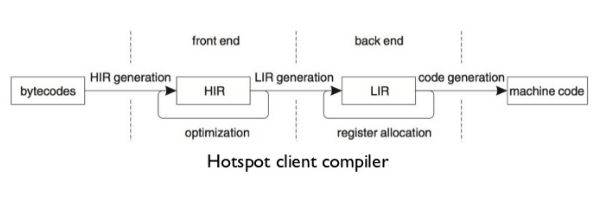
\includegraphics[scale = 0.4]
            {Images/concepts/crankshaft.png}
            \caption[crankshaft]%
            {V8 crankshaft\footnote{\url{http://www.slideshare.net/nwind/virtual-machine-and-javascript-engine/66-Builtin_objects_written_in_JSfunction}}}  
            \label{fig:crankshaft}
        \end{figure}
        
     As soon as these native machine code is produced, V8 engine will give fully access right of all data types, operators, objects and functions that described in ECMA standard to the browser or NodeJs to use them\textsuperscript{\ref{foot:v8Intro}}.   
     
     
    Moreover, there are three main reasons why V8 has a much higher performance than other JavaScript engines and that make V8 unique\textsuperscript{\ref{foot:v8git}}:
        \begin{enumerate}
            \item  Fast Property Access\newline
            V8 does not use dictionary-like data structure to store JavaScript properties as most of the other JavaScript engine does. Instead, it dynamically creates hidden classes, which eventually reduce the time required to access JavaScript properties\textsuperscript{\ref{foot:v8git}}.
            
            \item  Dynamic Machine Code Generation\newline
            As mentioned previously, when JavaScript source code is first executed, V8 compiles directly into machine. It means there are neither intermediate byte codes, nor interpreter, which is quite different from the other engines\textsuperscript{\ref{foot:v8git}}.
            
            \item  Efficient Garbage Collection\newline
            V8 reclaims memory used by objects that are no longer required in a process known as garbage collection. To ensure fast object allocation, short garbage collection pauses, and no memory fragmentation V8 employs a stop-the-world, generational, accurate, garbage collector\textsuperscript{\ref{foot:v8git}}.
        \end{enumerate}



        
    
    \subsection{Interface between JavaScript and C++}
        \subsubsection{FFI}
               
            Till now, we have talked about library, the structure mechanism of using a library (ABI). It's time to use that library from within JavaScript. One possible way to do that is using the FFI model of Node. Firstly, let's see what's FFI.
            
            \paragraph{What is FFI?} FFI refers to the ability for code written in one language, namely "host language," such as JavaScript, to access and invoke functions written in another language, namely the "guest language," such as C++\cite{Sigbjorn-99}.The reason why we call those functions "foreign" is because they come from another language and environment.\cite{Matthias-Grimmer-14}
            
            FFI access directly a library's binary code, which means it uses standard ABI to invoke functions in the library.
            
            \paragraph{Why FFI is good?} John Croisant, an experienced Ruby programmer, has shared 3 ideas of how to library written in lower-level languages, like C, within high-level languages, like Ruby.\footnote{\label{note1}\url{https://spin.atomicobject.com/2013/02/15/ffi-foreign-function-interfaces/}} They are:\newline
           
                \begin{itemize} 
                    \item \textit{1 Port all or part of the library to your language of choice.}
                    \item \textit{2 Write an extension in C code to bridge the gap between the library and your language.}
                    \item \textit{3 Wrap the library using your language's foreign function interface (FFI) support. }
                   \textsuperscript{\ref{note1}}\newline
                \end{itemize}
            
            So why FFI is the good? According to John, the major pops of FFI is its convenience to write and maintain compared with a C extension, its portability across platforms and language implementations, and it is easier for users to install. \textsuperscript{\ref{note1}}
            
            
            \paragraph{Node FFI}
            As you already know what FFI is, you can surely guess what Node FFI can do. I mention it here because on of the possible solution of our project is highly depending on this tool. Below is the definition given by the official documentation of Node FFI \textit{"node-ffi is a Node.js addon for loading and calling dynamic libraries using pure JavaScript. It can be used to create bindings to native libraries without writing any C++ code."} \footnote{\url{https://github.com/node-ffi/node-ffi}}


        \subsubsection{SWIG}
            \paragraph{What is SWIG?} The full name of SWIG is simplified wrapper and interface generator. It's a software that used to translate c and c++ files into scripting language or other languages. In the other word, it gives us the ability to call c and c++ files or programs or libraries from within other languages\footnote{\url{http://www.swig.org/}}.
            In fact, part of the job that SWIG does is quite similar to Node FFI. They all wrap functions written in low-level languages in order to invoke them in high-level languages. Plus, SWIG goes further. It can automatically generate shared libraries from source code and solves the problem of name mangling. Maybe there are something more. We will see. 
            
            \paragraph{Version 3.0 of SWIG}
            It's worth noting that from Version 3.0 of SWIG\footnote{\url{http://waywardmonkeys.org/2014/10/01/swig-and-javascript-part-one/}}, it began to support JavaScript. And that's how comes our second proposal. 



\begin{comment}
  A clear view of the advantages and disadvantages of the partial solutions found in the literature can be summarised by one or several tables (cf.\ table~\ref{tab:ProposalsComparison}) where a number of important criteria have been introduced and described.

Note that all figures, tables, and algorithms must be put into their corresponding floating environments, captioned, referenced from the main text, and sourced if they have been copied from previous work.
\end{comment}
  

\section{Conclusion}
In this chapter, we have gone through the basic conceptions of C++ compilation and JavaScript. We have introduced two tools, on which our proposal of this project will largely depend. One is Node FFI and the other is SWIG. In next chapter, general ideas of two proposals, namely possible solutions, of our project will be given.  
  
%--------------------------------------------------------------------------------

% \part{Proposals} % Commet it out if this has been done for the state-of-the-art
% \label{part:Proposa